\thispagestyle{empty}
\begin{center}
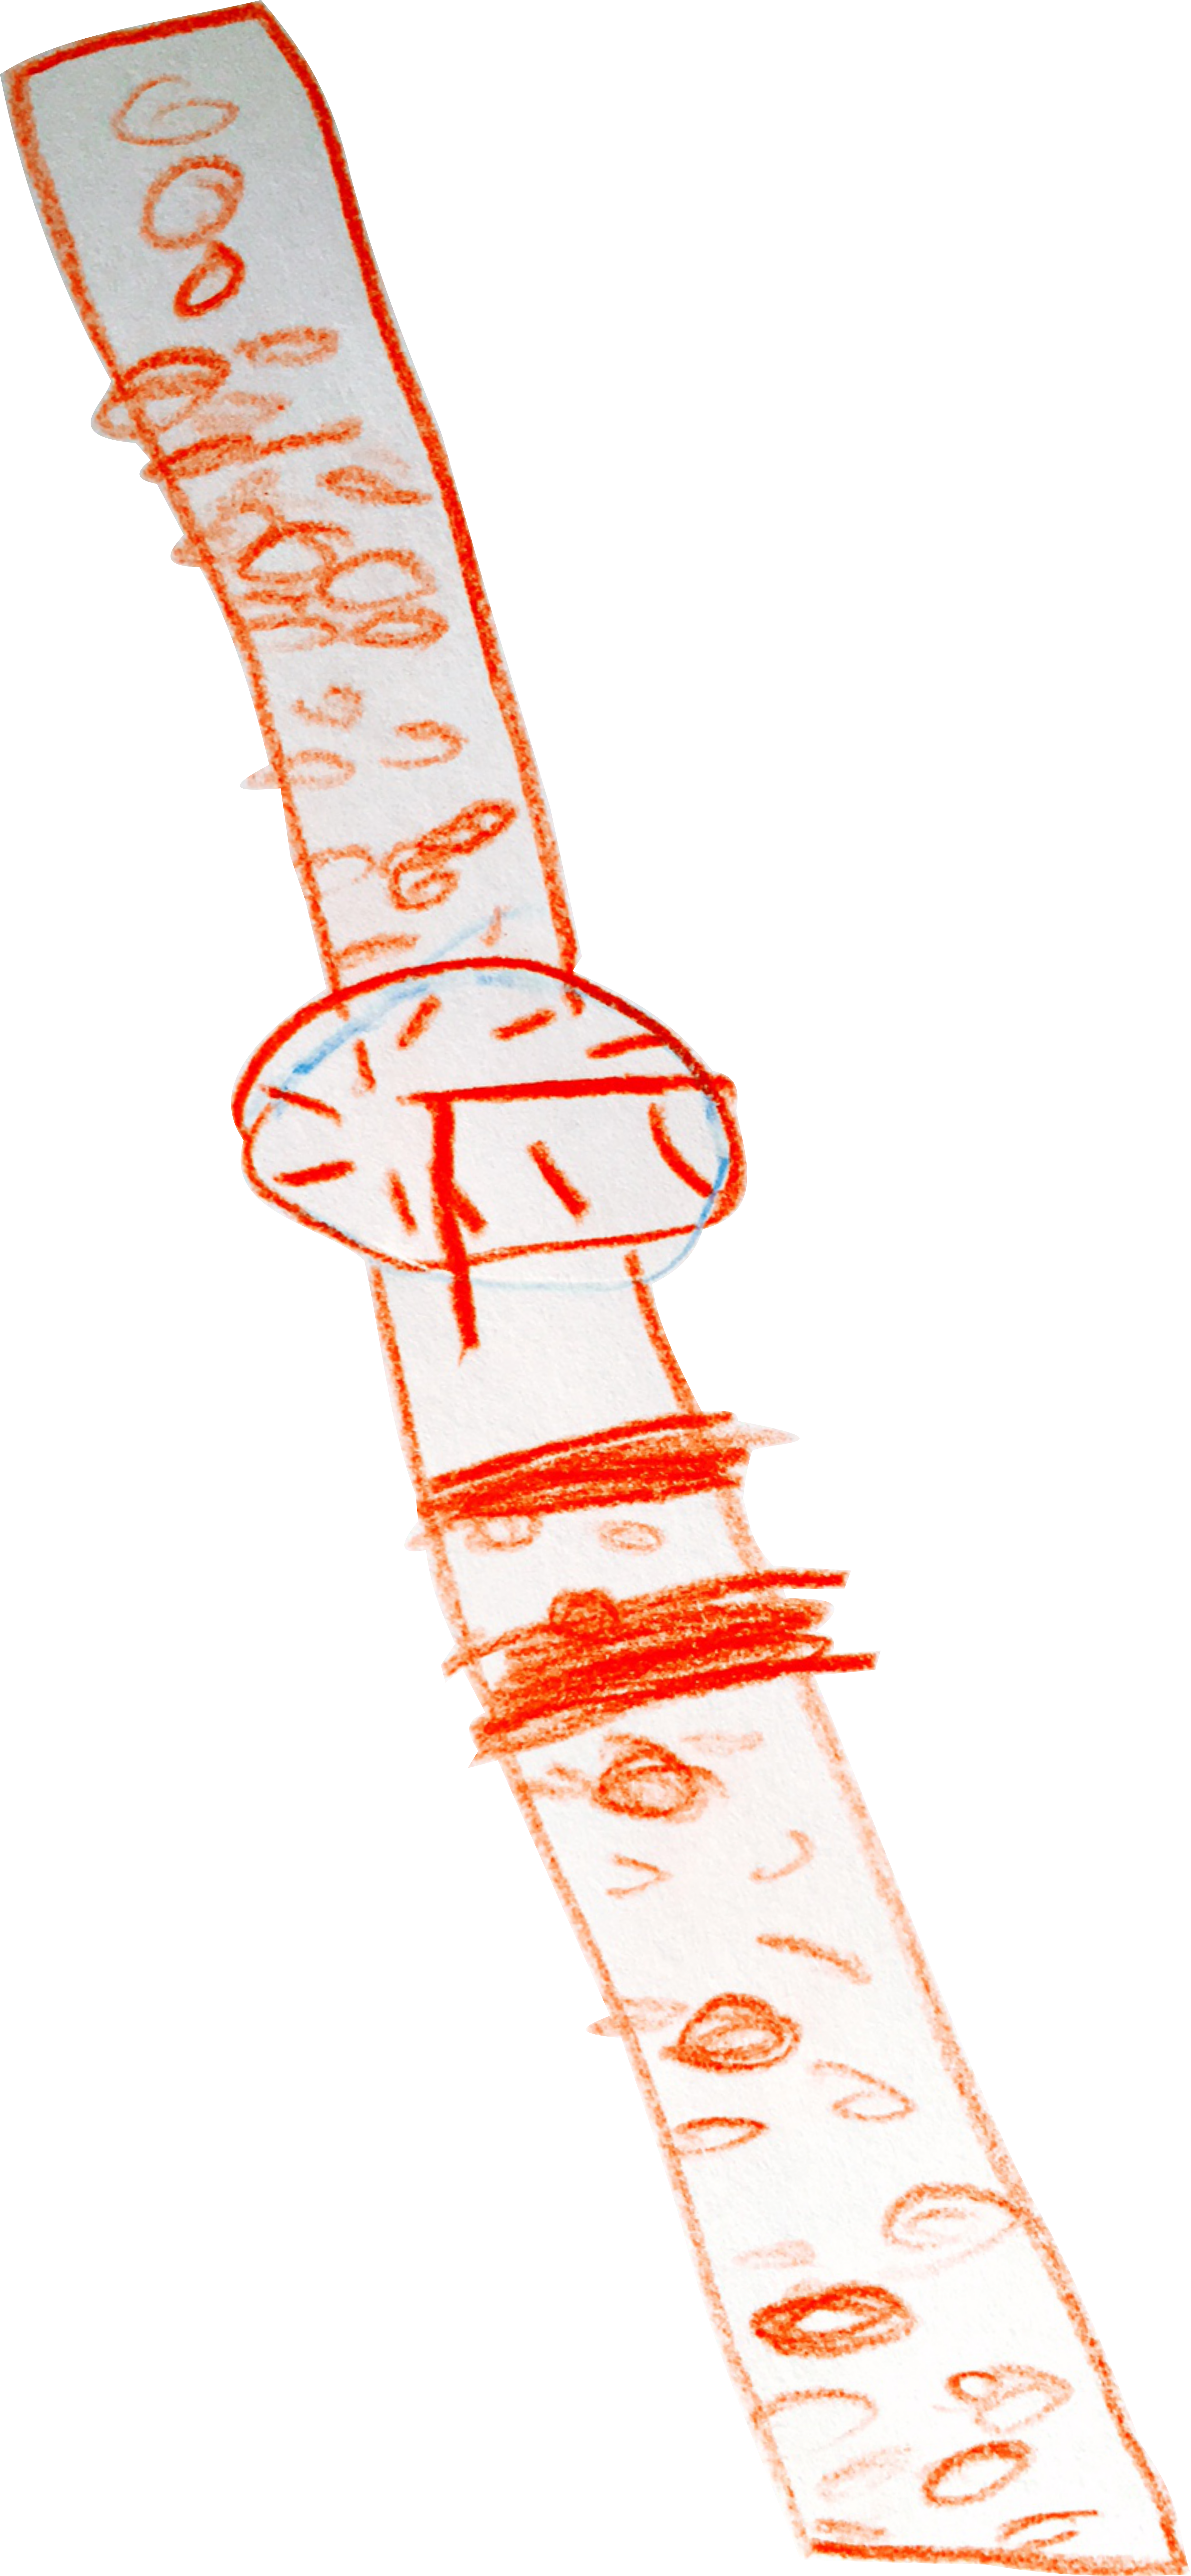
\includegraphics[height=.8\textheight]{./bilder/160120_uhr.png}
\end{center}
\vskip 2cm
{\Huge\color{farbe}\hfill{\ttfamily{Träume}}}
\addcontentsline{toc}{chapter}{Träume}
\newpage
%%%%%%%%%%%%%%%%%%%%%%%%%%%%%%%%%%%%%%%%%%%%%%%%%%%%%%%%%%%%%%%%%%%%%%%%%%%%%%%
\lettrine[lines=2, lhang=.2, loversize=.25, lraise=0.05, findent=0.1em,
nindent=0em]{A}{}ls ich ein Kind war, ich glaube, dass ich sieben oder acht
Jahre alt gewesen bin, da habe ich versucht zu träumen, dass ich im Traum
einschlafe und dann wiederum im Traum träume. Das habe ich mir über lange Zeit
jeden Abend vor dem Schlafen vorgenommen. Immer wieder. Und irgendwann hat es
tatsächlich geklappt.

Warum Menchen und auch einige Tiere träumen, weiss niemand. Alle Theorien dazu
sind -- nun ja -- eben Theorien und für mich nicht überzeugend. Für mich steht
fest, dass Träume und Phantasie sehr eng verwandt sind. Träume sind Phantasien,
nur dass man noch weniger aussuchen kann. Bei Phatasien kann man je wenigstens
das Thema wählen, aber was einem dann so in den Kopf kommt, weiss man ja vorher
auch nicht. 

Deswegen sagt man ja auch zum Beispiel \enquote{Ich habe den Traum, als erste
Kosmonautin Weltmeisterin im Riesenslalom zu werden und bei der Siegerehrung meinen
dritten Nummer eins Hit zu singen.} Diese Art von Traum, von Phantasie, ist
vermutlich der Motor für fast alles im Leben. Bei vielem von dem, was man tut oder macht,
stellen wir uns zuerst vor, was herauskommen soll. Ein Bild malen, den Beruf
aussuchen, eine Brücke bauen. Phantasien sind der Anfang.

Phantasien lassen alles zu. Ich darf mir vorstellen, wie es wohl wäre, zum
Beispiel den Sand vom Sandmännchen zu haben und dann jeden einschlafen lassen
zu können, wann ich will. Manchmal macht es auch Spass, Träume mit anderen zu
teilen. Deswegen werden Geschichten erzählt und Filme gedreht. Phantasien
werden erlebbar. 
\vfill

%Chrnopsychologie
%Philosophie der Zeit
%Bewegung
%Mechanik

